%% abtex2-modelo-trabalho-academico.tex, v-1.9.2 laurocesar
%% Copyright 2012-2014 by abnTeX2 group at http://abntex2.googlecode.com/ 
%%
%% This work may be distributed and/or modified under the
%% conditions of the LaTeX Project Public License, either version 1.3
%% of this license or (at your option) any later version.
%% The latest version of this license is in
%%   http://www.latex-project.org/lppl.txt
%% and version 1.3 or later is part of all distributions of LaTeX
%% version 2005/12/01 or later.
%%
%% This work has the LPPL maintenance status `maintained'.
%% 
%% The Current Maintainer of this work is the abnTeX2 team, led
%% by Lauro César Araujo. Further information are available on 
%% http://abntex2.googlecode.com/
%%
%% This work consists of the files abntex2-modelo-trabalho-academico.tex,
%% abntex2-modelo-include-comandos and abntex2-modelo-references.bib
%%

% ------------------------------------------------------------------------
% ------------------------------------------------------------------------
% abnTeX2: Modelo de Trabalho Academico (tese de doutorado, dissertacao de
% mestrado e trabalhos monograficos em geral) em conformidade com 
% ABNT NBR 14724:2011: Informacao e documentacao - Trabalhos academicos -
% Apresentacao
% ------------------------------------------------------------------------
% ------------------------------------------------------------------------

\documentclass[
	% -- opções da classe memoir --
	12pt,				% tamanho da fonte
	openright,			% capítulos começam em pág ímpar (insere página vazia caso preciso)
	twoside,			% para impressão em verso e anverso. Oposto a oneside
	a4paper,			% tamanho do papel. 
	% -- opções da classe abntex2 --
	%chapter=TITLE,		% títulos de capítulos convertidos em letras maiúsculas
	%section=TITLE,		% títulos de seções convertidos em letras maiúsculas
	%subsection=TITLE,	% títulos de subseções convertidos em letras maiúsculas
	%subsubsection=TITLE,% títulos de subsubseções convertidos em letras maiúsculas
	% -- opções do pacote babel --
	english,			% idioma adicional para hifenização
	french,				% idioma adicional para hifenização
	spanish,			% idioma adicional para hifenização
	brazil				% o último idioma é o principal do documento
	]{abntex2}

% ---
% Pacotes básicos 
% ---
\usepackage{lmodern}			% Usa a fonte Latin Modern			
\usepackage[T1]{fontenc}		% Selecao de codigos de fonte.
\usepackage[utf8]{inputenc}		% Codificacao do documento (conversão automática dos acentos)
\usepackage{lastpage}			% Usado pela Ficha catalográfica
\usepackage{indentfirst}		% Indenta o primeiro parágrafo de cada seção.
\usepackage{color}				% Controle das cores
\usepackage{graphicx}			% Inclusão de gráficos
\usepackage{microtype} 			% para melhorias de justificação
\usepackage[final]{pdfpages}
\usepackage{url}
\usepackage{float}
\usepackage{amsmath}
\usepackage{cleveref}
\usepackage{pgfplots}
\usepackage{amsfonts}
\usepackage{amsmath}
\usepackage{tikz}
\usetikzlibrary{matrix}

\DeclareMathOperator{\logsumexp}{logsumexp}
\pgfmathdeclarefunction{sumexp}{3}{%
  \begingroup%
  \pgfkeys{/pgf/fpu}% "/pgf/fpu/output format=fixed" removed
  \pgfmathsetmacro{\myx}{#1}%
  \pgfmathtruncatemacro{\myxmin}{#2}%
  \pgfmathtruncatemacro{\myxmax}{#3}%
  \pgfmathsetmacro{\mysum}{0}%
  \pgfplotsforeachungrouped\XX in {\myxmin,...,\myxmax}%
    {\pgfmathsetmacro{\mysum}{\mysum+exp(\XX)}}%
  \pgfmathparse{\mysum+exp(#1)}%
  \pgfmathfloattofixed\pgfmathresult%  added
  \pgfmathsmuggle\pgfmathresult\endgroup%
}

\crefname{figure}{Figura}{Figuras}
% ---
		
% ---
% Pacotes adicionais, usados apenas no âmbito do Modelo Canônico do abnteX2
% ---
\usepackage{lipsum}				% para geração de dummy text
% ---

% ---
% Pacotes de citações
% ---
\usepackage[brazilian,hyperpageref]{backref}	 % Paginas com as citações na bibl
\usepackage[alf]{abntex2cite}	% Citações padrão ABNT

% --- 
% CONFIGURAÇÕES DE PACOTES
% --- 

% ---
% Configurações do pacote backref
% Usado sem a opção hyperpageref de backref
\renewcommand{\backrefpagesname}{Citado na(s) página(s):~}
% Texto padrão antes do número das páginas
\renewcommand{\backref}{}
% Define os textos da citação
\renewcommand*{\backrefalt}[4]{
	\ifcase #1 %
		Nenhuma citação no texto.%
	\or
		Citado na página #2.%
	\else
		Citado #1 vezes nas páginas #2.%
	\fi}%
% ---

% ---
% Informações de dados para CAPA e FOLHA DE ROSTO
% ---
\titulo{Geração procedural de mapas de ilhas 2d com biomas através de técnicas de segmentação de imagem}
\autor{Lucas da Silva dos Santos\\Matheus Zanivan Andrade\\ Rafael Nascimento Lourenço}
\local{São Paulo - Brasil}
\data{2023}
\orientador{Lauro César Araujo}
\coorientador{Equipe \abnTeX}
\instituicao{%
  Senac: Serviço Nacional de Aprendizagem Comercial
  \par
  Bacharelado em ciência da computação
}
\tipotrabalho{Trabalho de Conclusão de Curso (TCC)}
% O preambulo deve conter o tipo do trabalho, o objetivo, 
% o nome da instituição e a área de concentração 
\preambulo{Modelo canônico de trabalho monográfico acadêmico em conformidade com
as normas ABNT apresentado à comunidade de usuários \LaTeX.}
% ---


% ---
% Configurações de aparência do PDF final

% alterando o aspecto da cor azul
\definecolor{blue}{RGB}{41,5,195}

% informações do PDF
\makeatletter
\hypersetup{
     	%pagebackref=true,
		pdftitle={\@title}, 
		pdfauthor={\@author},
    	pdfsubject={\imprimirpreambulo},
	    pdfcreator={LaTeX with abnTeX2},
		pdfkeywords={abnt}{latex}{abntex}{abntex2}{trabalho acadêmico}, 
		colorlinks=true,       		% false: boxed links; true: colored links
    	linkcolor=blue,          	% color of internal links
    	citecolor=blue,        		% color of links to bibliography
    	filecolor=magenta,      		% color of file links
		urlcolor=blue,
		bookmarksdepth=4
}
\makeatother
% --- 

% --- 
% Espaçamentos entre linhas e parágrafos 
% --- 

% O tamanho do parágrafo é dado por:
\setlength{\parindent}{1.3cm}

% Controle do espaçamento entre um parágrafo e outro:
\setlength{\parskip}{0.2cm}  % tente também \onelineskip

% ---
% compila o indice
% ---
\makeindex
% ---

% ----
% Início do documento
% ----
\begin{document}

% Retira espaço extra obsoleto entre as frases.
\frenchspacing 

% ----------------------------------------------------------
% ELEMENTOS PRÉ-TEXTUAIS
% ----------------------------------------------------------
% \pretextual

% ---
% Capa
% ---
\imprimircapa
% ---

% ---
% Folha de rosto
% (o * indica que haverá a ficha bibliográfica)
% ---
\imprimirfolhaderosto*
% ---

% ---
% Inserir a ficha bibliografica
% ---
% Isto é um exemplo de Ficha Catalográfica, ou ``Dados internacionais de
% catalogação-na-publicação''. Você pode utilizar este modelo como referência. 
% Porém, provavelmente a biblioteca da sua universidade lhe fornecerá um PDF
% com a ficha catalográfica definitiva após a defesa do trabalho. Quando estiver
% com o documento, salve-o como PDF no diretório do seu projeto e substitua todo
% o conteúdo de implementação deste arquivo pelo comando abaixo:
%
\begin{fichacatalografica}
    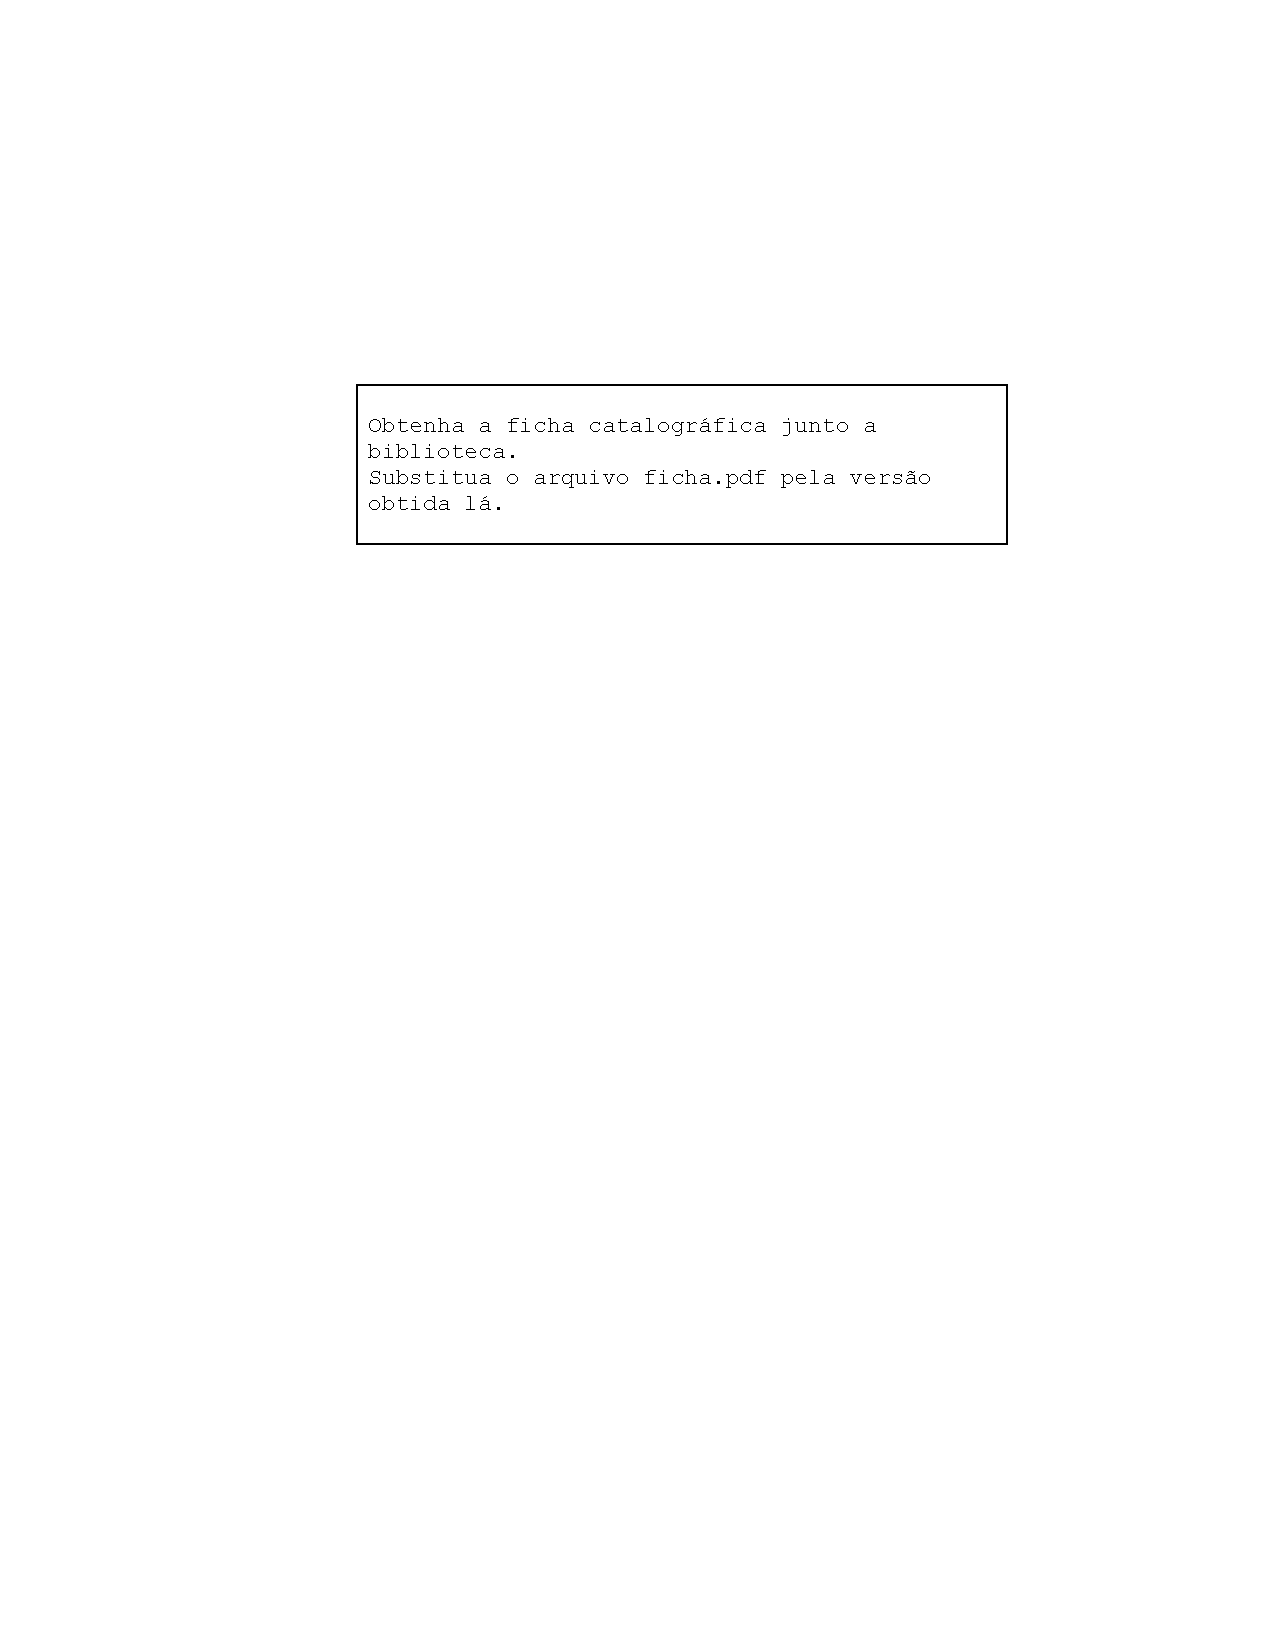
\includepdf{ficha.pdf}
\end{fichacatalografica}
% ---

% ---
% Inserir errata
% ---
% \begin{errata}
% Elemento opcional da \citeonline[4.2.1.2]{NBR14724:2011}. Exemplo:

% \vspace{\onelineskip}

% FERRIGNO, C. R. A. \textbf{Tratamento de neoplasias ósseas apendiculares com
% reimplantação de enxerto ósseo autólogo autoclavado associado ao plasma
% rico em plaquetas}: estudo crítico na cirurgia de preservação de membro em
% cães. 2011. 128 f. Tese (Livre-Docência) - Faculdade de Medicina Veterinária e
% Zootecnia, Universidade de São Paulo, São Paulo, 2011.

% \begin{table}[htb]
% \center
% \footnotesize
% \begin{tabular}{|p{1.4cm}|p{1cm}|p{3cm}|p{3cm}|}
%   \hline
%    \textbf{Folha} & \textbf{Linha}  & \textbf{Onde se lê}  & \textbf{Leia-se}  \\
%     \hline
%     1 & 10 & auto-conclavo & autoconclavo\\
%    \hline
% \end{tabular}
% \end{table}

% \end{errata}
% ---

% ---
% Inserir folha de aprovação
% ---

% Isto é um exemplo de Folha de aprovação, elemento obrigatório da NBR
% 14724/2011 (seção 4.2.1.3). Você pode utilizar este modelo até a aprovação
% do trabalho. Após isso, substitua todo o conteúdo deste arquivo por uma
% imagem da página assinada pela banca com o comando abaixo:
%
% \includepdf{folhadeaprovacao_final.pdf}
%
\begin{folhadeaprovacao}

  \begin{center}
    {\ABNTEXchapterfont\large\imprimirautor}

    \vspace*{\fill}\vspace*{\fill}
    \begin{center}
      \ABNTEXchapterfont\bfseries\Large\imprimirtitulo
    \end{center}
    \vspace*{\fill}
    
    \hspace{.45\textwidth}
    \begin{minipage}{.5\textwidth}
        \imprimirpreambulo
    \end{minipage}%
    \vspace*{\fill}
   \end{center}
        
%    Trabalho aprovado. \imprimirlocal, 24 de novembro de 2012:

   \assinatura{\textbf{\imprimirorientador} \\ Orientador} 
   \assinatura{\textbf{Professor} \\ Convidado 1}
   \assinatura{\textbf{Professor} \\ Convidado 2}
   %\assinatura{\textbf{Professor} \\ Convidado 3}
   %\assinatura{\textbf{Professor} \\ Convidado 4}
      
   \begin{center}
    \vspace*{0.5cm}
    {\large\imprimirlocal}
    \par
    {\large\imprimirdata}
    \vspace*{1cm}
  \end{center}
  
\end{folhadeaprovacao}
% ---

% ---
% Dedicatória
% ---
\begin{dedicatoria}
   \vspace*{\fill}
   \centering
   \noindent
   \textit{ Este trabalho é dedicado às crianças adultas que,\\
   quando pequenas, sonharam em se tornar cientistas.} \vspace*{\fill}
\end{dedicatoria}
% ---

% ---
% Agradecimentos
% ---
\begin{agradecimentos}
Os agradecimentos principais são direcionados à Gerald Weber, Miguel Frasson,
Leslie H. Watter, Bruno Parente Lima, Flávio de Vasconcellos Corrêa, Otavio Real
Salvador, Renato Machnievscz\footnote{Os nomes dos integrantes do primeiro
projeto abn\TeX\ foram extraídos de
\url{http://codigolivre.org.br/projects/abntex/}} e todos aqueles que
contribuíram para que a produção de trabalhos acadêmicos conforme
as normas ABNT com \LaTeX\ fosse possível.

Agradecimentos especiais são direcionados ao Centro de Pesquisa em Arquitetura
da Informação\footnote{\url{http://www.cpai.unb.br/}} da Universidade de
Brasília (CPAI), ao grupo de usuários
\emph{latex-br}\footnote{\url{http://groups.google.com/group/latex-br}} e aos
novos voluntários do grupo
\emph{\abnTeX}\footnote{\url{http://groups.google.com/group/abntex2} e
\url{http://abntex2.googlecode.com/}}~que contribuíram e que ainda
contribuirão para a evolução do \abnTeX.

\end{agradecimentos}
% ---

% ---
% Epígrafe
% ---
\begin{epigrafe}
    \vspace*{\fill}
	\begin{flushright}
		\textit{``Não vos amoldeis às estruturas deste mundo, \\
		mas transformai-vos pela renovação da mente, \\
		a fim de distinguir qual é a vontade de Deus: \\
		o que é bom, o que Lhe é agradável, o que é perfeito.\\
		(Bíblia Sagrada, Romanos 12, 2)}
	\end{flushright}
\end{epigrafe}
% ---

% ---
% RESUMOS
% ---

% resumo em português
% \setlength{\absparsep}{18pt} % ajusta o espaçamento dos parágrafos do resumo
% \begin{resumo}
%  Segundo a \citeonline[3.1-3.2]{NBR6028:2003}, o resumo deve ressaltar o
%  objetivo, o método, os resultados e as conclusões do documento. A ordem e a extensão
%  destes itens dependem do tipo de resumo (informativo ou indicativo) e do
%  tratamento que cada item recebe no documento original. O resumo deve ser
%  precedido da referência do documento, com exceção do resumo inserido no
%  próprio documento. (\ldots) As palavras-chave devem figurar logo abaixo do
%  resumo, antecedidas da expressão Palavras-chave:, separadas entre si por
%  ponto e finalizadas também por ponto.

%  \textbf{Palavras-chaves}: latex. abntex. editoração de texto.
% \end{resumo}

% resumo em inglês
% \begin{resumo}[Abstract]
%  \begin{otherlanguage*}{english}
%    This is the english abstract.

%    \vspace{\onelineskip}
 
%    \noindent 
%    \textbf{Key-words}: latex. abntex. text editoration.
%  \end{otherlanguage*}
% \end{resumo}
% ---

% ---
% inserir lista de ilustrações
% ---
% \pdfbookmark[0]{\listfigurename}{lof}
% \listoffigures*
% \cleardoublepage
% ---

% ---
% inserir lista de tabelas
% ---
% \pdfbookmark[0]{\listtablename}{lot}
% \listoftables*
% \cleardoublepage
% ---

% ---
% inserir lista de abreviaturas e siglas
% ---
% \begin{siglas}
%   \item[ABNT] Associação Brasileira de Normas Técnicas
%   \item[abnTeX] ABsurdas Normas para TeX
% \end{siglas}
% ---

% ---
% inserir lista de símbolos
% ---
% \begin{simbolos}
%   \item[$ \Gamma $] Letra grega Gama
%   \item[$ \Lambda $] Lambda
%   \item[$ \zeta $] Letra grega minúscula zeta
%   \item[$ \in $] Pertence
% \end{simbolos}
% ---

% ---
% inserir o sumario
% ---
\pdfbookmark[0]{\contentsname}{toc}
\tableofcontents*
\cleardoublepage
% ---



% ----------------------------------------------------------
% ELEMENTOS TEXTUAIS
% ----------------------------------------------------------
\textual

% ----------------------------------------------------------
% Introdução (exemplo de capítulo sem numeração, mas presente no Sumário)
% ----------------------------------------------------------
\chapter[Introdução]{Introdução}
% ----------------------------------------------------------
\section{Contexto}

A indústria de jogos digitais cresce mais a cada dia, segundo a consultora Newzoo \space\cite{quanto_games_vao_movimentar} essa indústria tende a ultrapassar em 2023 os US\$ 200 bilhões (aproximadamente R\$ 1 trilhão). Novos jogos são produzidos e publicados diariamente e somente na plataforma digital Steam, foram publicados 10.963 novos títulos em 2022\space
\cite{numero_de_jogos_publicados_na_steam}.

Ademais, as empresas de desenvolvimento de jogos continuam a trabalhar incessantemente para atender a uma demanda de mercado que cresceu 2,5\% no Brasil em 2022 
\space
\cite{pesquisa_games_brasil}. O custo de produção de jogos varia bastante, dependendo do tamanho e da complexidade do projeto, \emph{e.g.}, a empresa Rockstar Games revelou que o jogo \"Grand Theft Auto V\" custou cerca de 265 milhões de dólares para ser produzido e comercializado \space
\cite{gta_quanto_custou}.

Outro cenário que está crescendo muito nos últimos anos é o da inteligência artificial afirma \citeonline{Valente_2020} que no Brasil mais que dobrou o número contratações de desenvolvedores da área de 2015 até 2020. De acordo com \apud{johnson2023}{briggs2023} um relatório recente relata que 300 milhões de empregos podem ser afetados pela IA \emph{i.e.} 18\% ofício global pode ser automatizado. Outrossim \citeonline{europarl2020} diz que o tópico de inteligência artificial é uma prioridade para União Europeia por ser considerada primordial para transformação digital da sociedade.  Do mesmo modo, "Bill Gates, um dos fundadores da Microsoft — uma das maiores empresas de tecnologia —, diz que o desenvolvimento da inteligência artificial (IA) é o avanço tecnológico mais importante em décadas"\space
\cite{inteligencia_artificial_e_avanco_bbc}.

\section{Justificativa}

O mapa é um elemento que se destaca em jogos digitais e pode ser criado usando técnicas de geração procedural de conteúdo, porém existe um desafio em criar cenários bonitos e diversificados \cite{geracao_procedural_jogos_2d}.

Segundo \citeonline{diagrama_voronoi_jogos}, a área de Geometria Computacional é um ramo da ciência da computação que estuda algoritmos e estruturas de dados para resolução computacional de problemas geométricos e o diagrama de Voronoi é um dos tópicos mais discutidos dessa área. O diagrama de Voronoi pode ser utilizado para resolver alguns problemas relacionados à jogos como por exemplo marcar pontos no mapa e desses pontos criar regiões, a partir dessas regiões criar biomas para serem usados no algoritmo de geração procedural de conteúdo para criar mapas.

De acordo com \citeonline{jogo_procedural} é muito comum em jogos usar técnicas procedurais para otimizar o processo de criação além de ser comum o uso conjunto de inteligência artificial para melhorar ou personalizar como o jogo RimWorld que um simulador conduzido por uma IA que gera histórias no modo procedural.

Dito isso, nosso projeto tem a ideia de fornecer recursos baseados em matemática aplicada dentro de ciência da computação que proporcione uma funcionalidade  de escolher o contorno do mapa no qual irá jogar através de imagens. Abordaremos a arquitetura de redes neurais convolucionais, que é muito utilizada para trabalhar com imagens. Mais especificamente, abordaremos uma arquitetura derivada da anteriormente citada, específica para segmentação de imagens, o que possibilita reconhecer contornos em imagens. Complementando que IA não é a única maneira de encontrar bordas em imagens, contemplaremos outras técnicas específicas de segmentação de imagem.

Adicionando a isso por definição o conceito de ilha é terra cercada de água, logo a única diferença para um continente é o seu tamanho, baseando-se nisso, a escolha de ser uma ilha é porque é uma opção generalista utilizada em diversos jogos como Grand Theft Auto V, Just Cause 4, Fortnite, Pokémon Scarlet \& Violet, dentre outros. Acrescentando sobre a decisão de criar mapas 2D, é pontuado que há uma complexidade enorme entre mapas de 2D e 3D e que não é o foco proposto para o trabalho em questão. 

\section{Objetivos}

O objetivo geral deste trabalho explora técnicas e algoritmos que permeiam os ramos de inteligência artificial com foco em identificar contornos em imagens e computação 
gráfica centrado em gerar mapas usando heurísticas.
Ademais visto especificamente temos como objetivos:

\begin{itemize}
	\item Encontrar um dataset para treinar a inteligência artificial que irá identificar contornos em imagens
	\item Treinar uma inteligência artificial para identificar contornos em imagens
	\item Testar algoritmos de gerar ruídos para criar o mapa
	\item Aplicar um algoritmo para reconhecer a imagem com o contorno e gerar como saída a imagem do mapa gerado
\end{itemize}


\chapter{Fundamentação teórica}
\label{sec:background}
	\label{sec:fund_teorica}

Este capítulo tem objetivo de apresentar conceitos necessários para entendimento do trabalho.

\section{Inteligência Artificial}
Inteligência artificial é uma técnica científica que simula o pensamento humano de forma que possa ser executado em uma máquina, podendo ser utilizada para criar soluções com uma linha de progressão parecida ao raciocínio lógico como conhecemos. Isto permite ao computador reconhecer e interpretar o mundo ao redor com imagens e textos criando uma ampla área de atuação que otimiza tarefas antes só realizadas por seres humanos \space\cite{ia_aliada_ou_inimiga}.

Este ramo é complexo por se tratar de uma representação cognitiva, se torna necessário usar uma base com diversas áreas científicas como psicologia, biologia, lógica matemática, linguística, engenharia, filosofia, entre outras. E pode ser usado para diversos problemas específicos como, por exemplo, definir as boas rotas para algum processo logístico \space\cite{ia_conceitos_aplicacoes}.

\begin{figure}[H]
	\caption{Diagrama de aprendizado de máquina}
	\centering % para centralizarmos a figura
	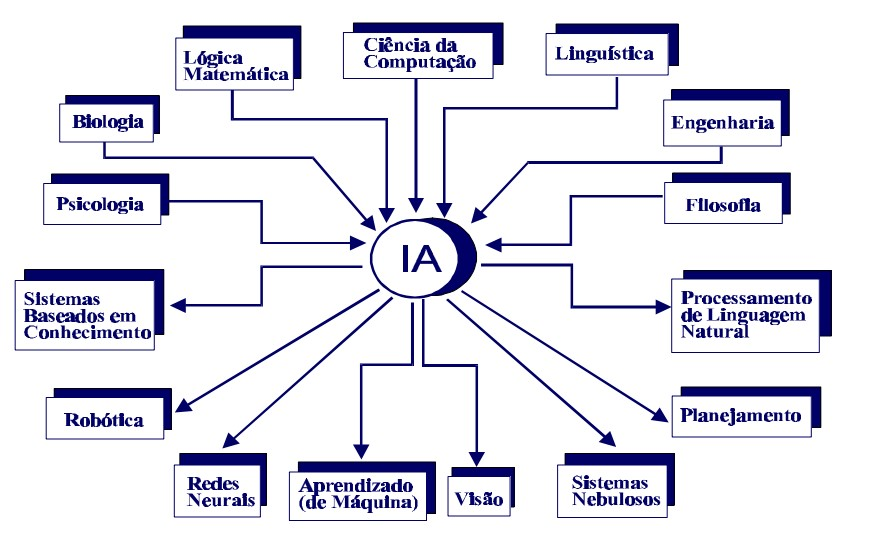
\includegraphics[width=10cm]{figures/areas_ia.jpg} % leia abaixo
	\legend{Fonte: \citeonline{aplicacoes_ia_vg}}
	\label{fig:areas_ia}
\end{figure}

Segundo \citeonline{dp_overview} existe três tópicos sobre inteligência artificial muito populares sendo eles, inteligência artificial, aprendizado de máquina e aprendizado profundo como segue na imagem \cref{fig:diagrama_ia_ml_dp}.

\begin{figure}[H]
	\caption{Diagrama de Venn sobre relação entre os tópicos de inteligência artificial}
	\centering % para centralizarmos a figura
	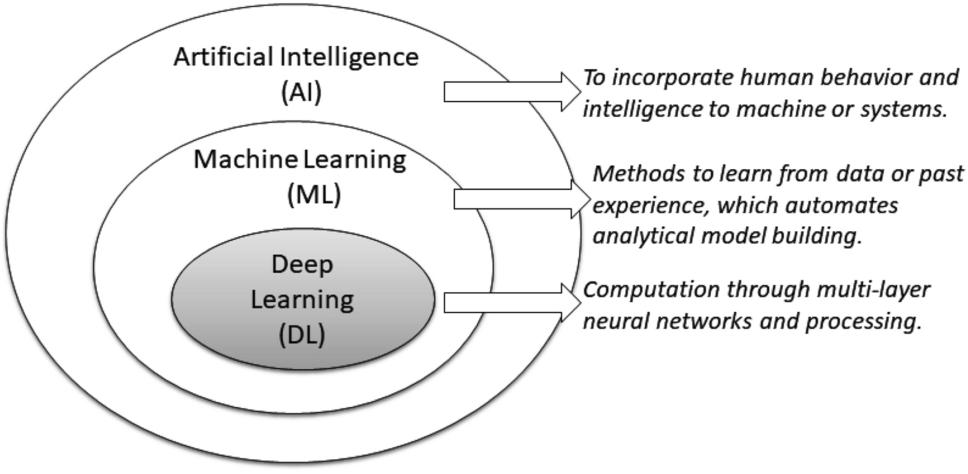
\includegraphics[width=10cm]{figures/diagrama_ia_ml_dp.png} % leia abaixo
	\legend{Fonte: \citeonline{dp_overview}}
	\label{fig:diagrama_ia_ml_dp}
\end{figure}

\subsection{Aprendizado de Máquina}


Segundo \citeonline{directions_ia_ml_dp}, aprendizado de máquina é uma subcategoria de inteligência artificial que se refere  a detecção de padrões importantes de uma base de dados. As ferramentas utilizadas aumentam a eficiência dos algoritmos para lidar com bases de dados grandes.

Portanto, essa técnica permite ao computador melhorar os resultados com base na experiência, isso indica uma relação direta entre o quanto o programa consumiu de dados e qualidade da solução do problema \cite{ml_explicado}. 

Dentro desse nicho existem outros como: redes neurais, algoritmos evolucionários, algoritmos de busca, aprendizado por reforço, dentre outros. \cite{ml_oil_gas_industry}.

Existe relação direta de conceitos entre inteligência artificial, aprendizado de máquina e ciência de dados conforme mostrado na \cref{fig:diagrama_ia}.

\begin{figure}[H]
	\caption{Diagrama de aprendizado de máquina}
	\centering % para centralizarmos a figura
	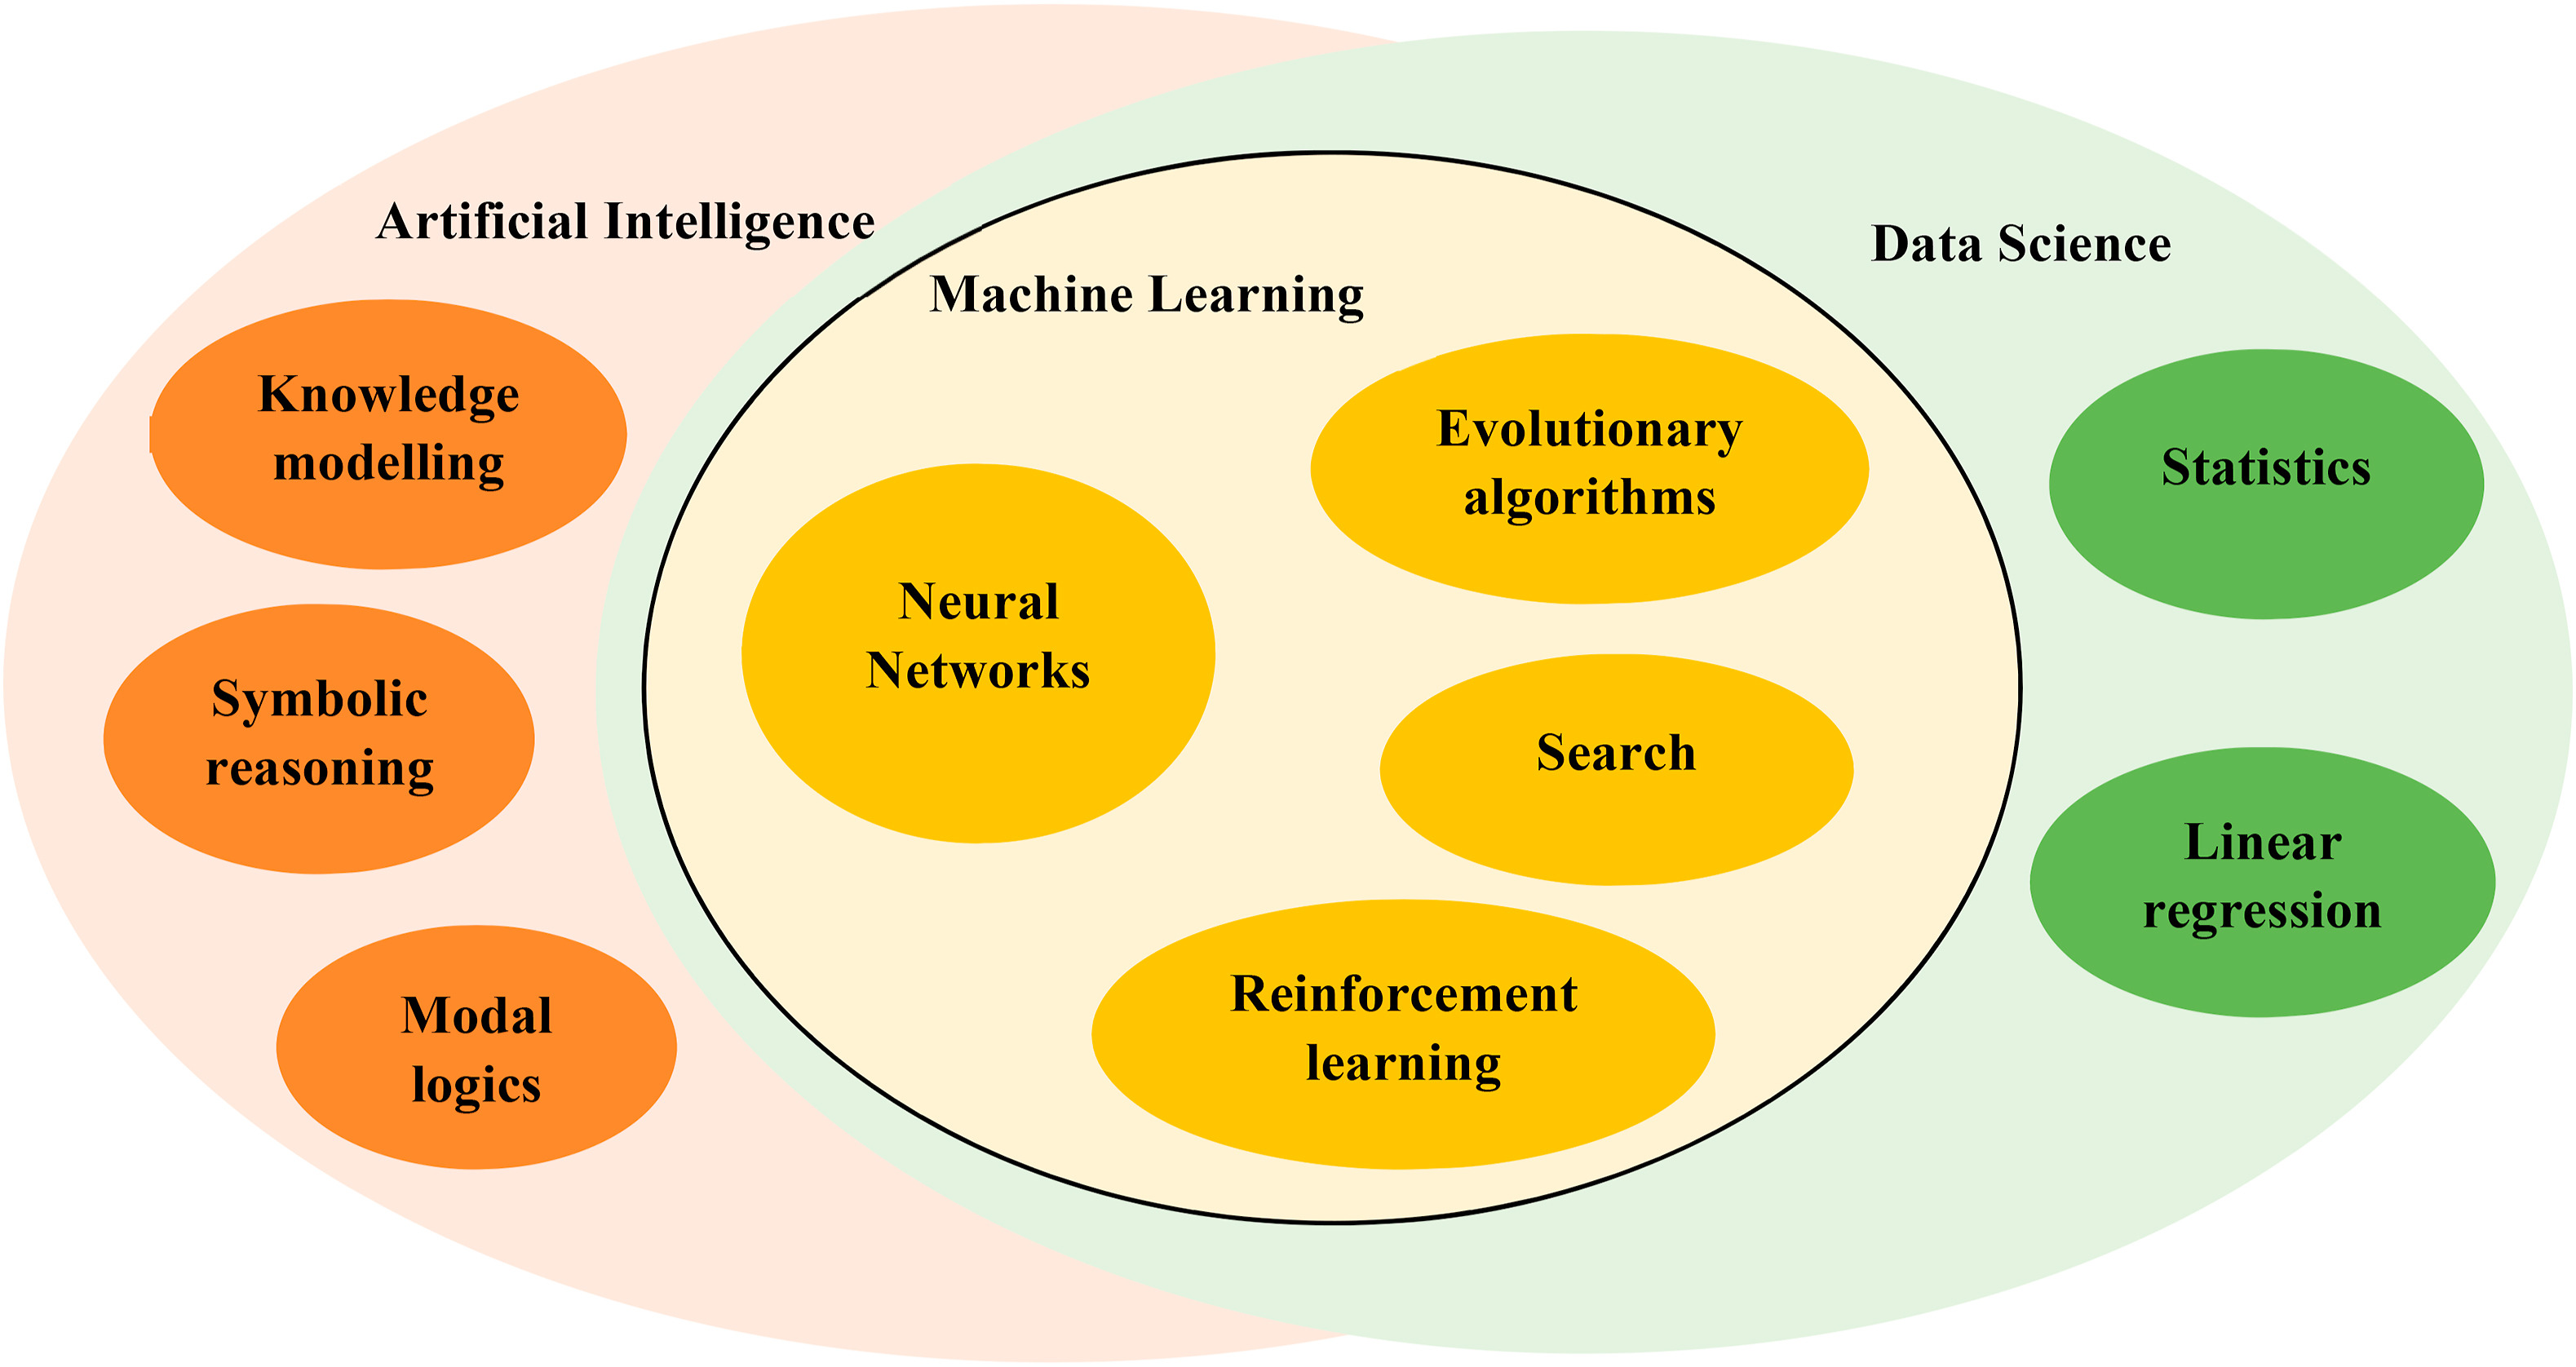
\includegraphics[width=10cm]{figures/diagrama_ia.jpg} % leia abaixo
	\legend{Fonte: \citeonline{ml_oil_gas_industry}}
	\label{fig:diagrama_ia}
\end{figure}

É possível observar uma hierarquia entre aprendizado de máquina e os principais termos sendo eles redes neurais artificiais e aprendizado profundo com base em \citeonline{ml_and_dp} mostrado no diagrama da \cref{fig:diagrama_ann}.

\begin{figure}[H]
	\caption{Diagrama de Venn sobre tópicos de aprendizado de máquina}
	\centering % para centralizarmos a figura
	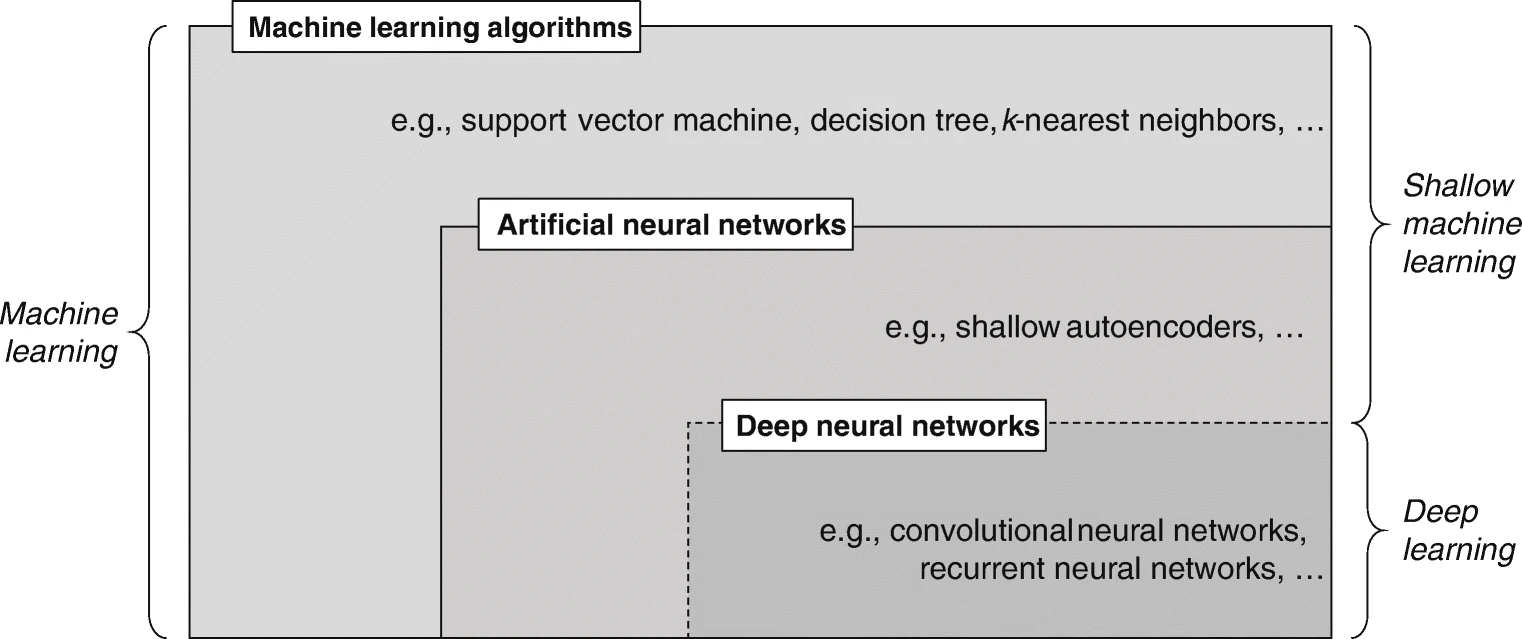
\includegraphics[width=10cm]{figures/diagrama_ann.jpg} % leia abaixo
	\legend{Fonte: \citeonline{ml_and_dp}}
	\label{fig:diagrama_ann}
\end{figure}

\subsubsection{Rede neural artificial}

Uma rede neural artificial é uma representação matemática de unidades de processamento conectadas chamadas de neurônios artificiais . Essa arquitetura simula sinapses, cada sinal trocado entre os neurônios pode aumentar ou atenuar os sinais de outros durante o aprendizado\cite{ml_and_dp}.
\begin{figure}[H]
	\centering
	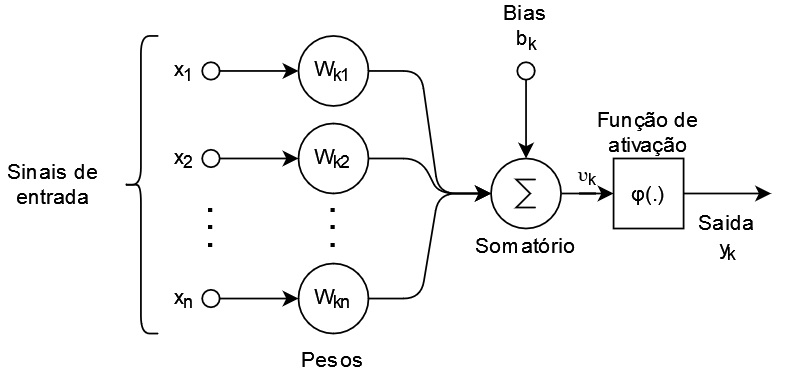
\includegraphics[width=0.8\textwidth]{figures/neuronio.png}
	\caption{Modelo de um neurônio não-linear \cite{haykin1999neural}.}
	\label{fig:neuronio}
\end{figure}

Observando a figura \ref{fig:neuronio} vemos o funcionamento de um neurônio $k$. Os sinais de entradas são partes de um vetor $x$ de tamanho $n$, sendo o vetor composto por $x_1, x_2 ... x_n$, essas componentes são combinadas em uma soma ponderada utilizando seus respectivos pesos, $w_{k1}, w_{k2}...w_{kn}$, formando assim a seguinte equação  \apud{marti2017aprendizado}{haykin1999neural}:

$$\upsilon_k = \sum_{i=1}^n (x_i * w_{ki})$$

O resultado dessa equação produz o potencial de ativação $\upsilon_k$, esse resultado é somado com o \textit{bias} ou viés $b_k$ para manipular a saída $y_k$ do neurônio, essa soma é posta em uma função não-linear nomeada de função de ativação $\varphi(.)$, essas funções mapeiam a saída em um intervalo $[0, 1]$ ou $[1, -1]$. A função de saída pode ser representada com a seguinte equação \apud{marti2017aprendizado}{haykin1999neural}:

$$y_k = \varphi(\upsilon_k + b_k)$$

O aprendizado ocorre na faze de treinamento onde é ajustando os pesos $w_k$ e o viés $b_k$ de cada neurônio $k$. Os pesos $w_k$ são utilizados para calcular a taxa de crescimento da função e o viés $b_k$ é necessário para descolar a saída da função. Com isso é possível modelar uma função linear $y=w^T*x+b$ \cite{marti2017aprendizado}.

Para cada amostra o modelo compara os resultados dos valores atuais dos pesos $w_k$ e viés $b_k$ com o resultado esperado(alvo). Uma função custo(\textit{cost function}) é utilizada para gerar um vetor de gradientes e para quantificar o erro encontrado para a configuração atual do modelo. O modelo atualiza os pesos $w_k$ e os viés $b_k$ no sentido contrário do vetor de gradientes, buscando minimizar a função de custo de acordo com uma taxa de aprendizado(\textit{learning rate}) \cite{marti2017aprendizado}.

Ao combinar diversos neurônios artificiais forma-se uma rede neural Artificial. Essas redes buscam simular o processamento de informação do cérebro humano \cite{ferneda2006redes}.
Nas redes neurais os neurônios são organizados em grupos de unidade de processamento chamados camadas. A primeira e a última camada são nomeadas de camada de entrada e camada de saída e as demais de camadas ocultas. As camadas mais próximas da entrada são responsáveis por identificar características mais primitivas e as seguintes combinam essas informações para identificar padrões mais complexos \cite{marti2017aprendizado}.

\subsubsection{Funções de ativação}

Nas redes neurais os neurônios são organizados em grupos de unidade de processamento chamados camadas. A primeira e a ultima camada são nomeadas de camada de entrada e camada de saída e as demais de camadas ocultas. As camadas mais próximas da entrada são responsáveis por identificar características mais primitivas e as seguintes combinam essas informações para identificar padrões mais complexos \cite{marti2017aprendizado}.

\subsubsection{Funções de ativação}

A função de ativação retorna a saída de um neurônio \cite{haykin1999neural}, aqui podemos ver três tipos de funções de ativação:

\begin{enumerate}
	\item Função \textit{Sigmoid}, uma função não-linear que produz uma curva com a forma de "S". Usada para mapear valores previstos em probabilidades. Tem o valor de saída entre 0 e 1 \cite{gharat2019what}.
	\begin{figure}[H]
	\begin{center}
		\begin{minipage}{0.45\textwidth}
			$$\varphi(\upsilon) = \frac{1}{1 + e^{-\upsilon}}$$
		\end{minipage}
		\hfill
		\begin{minipage}{0.45\textwidth}
			\begin{tikzpicture}
				\begin{axis}[
					width=0.9\textwidth,
					height=0.7\textwidth,
					xlabel={$\upsilon$},
					xmin=-6, xmax=6,
					ymin=0, ymax=1,
				]
					\addplot[
						color=red,
						domain=-6:6,
					] {1/(1+exp(-x))};
				\end{axis}
			\end{tikzpicture}
		\end{minipage}
	\end{center}
	\caption{Gráfico da função \textit{Sigmoid}.}
	\label{fig:grafico_sigmoid}
	\end{figure}

	\item Função \textit{ReLu} (Unidade Linear Retificada), função não-linear inspirada nos neurônios do cérebro que retorna um valor positivo ou 0 \cite{rizzo2020inteligencia}.
	\begin{figure}[H]
	\begin{center}
		\begin{minipage}{0.45\textwidth}
			$$\varphi(\upsilon) = \max(0,\upsilon)$$
		\end{minipage}
		\hfill
		\begin{minipage}{0.45\textwidth}
			\begin{tikzpicture}
				\begin{axis}[
					width=0.9\textwidth,
					height=0.7\textwidth,
					xlabel={$\upsilon$},
					xmin=-6, xmax=6,
					ymin=0, ymax=5,
				]
					\addplot[red, domain=-5:0] {0};
					\addplot[red, domain=0:5] {x};
				\end{axis}
			\end{tikzpicture}
		\end{minipage}
	\end{center}
	\caption{Gráfico da função \textit{ReLu}.}
	\label{fig:grafico_relu}
	\end{figure}

	\item Função \textit{Softmax}, calcula a distribuição de probabilidades de um evento em "n" eventos e fornece a probabilidade do valor de entrada pertencer a uma classe específica, geralmente usada na camada de saída \cite{gharat2019what}.
	\begin{figure}[H]
	\begin{center}
		\begin{minipage}{0.45\textwidth}
			$$\varphi(\upsilon) = \frac{e^{\upsilon_i}}{\sum_{j=0} e^{\upsilon_i}}$$
		\end{minipage}
		\hfill
		\begin{minipage}{0.45\textwidth}
			\begin{tikzpicture}
				\begin{axis}[
					width=0.9\textwidth,
					height=0.7\textwidth,
					xlabel={$\upsilon$},
					xmin=-10, xmax=10,
					ymin=0, ymax=1,
				]
					\addplot[red,domain=-10:10,samples=51] {exp(x)/sumexp(x,-4,0)};
				\end{axis}
			\end{tikzpicture}
		\end{minipage}
	\end{center}
	\caption{Gráfico da função \textit{Softmax}.}
	\label{fig:grafico_softmax}
	\end{figure}
\end{enumerate}



\subsection{Aprendizado profundo}

O aprendizado profundo é uma área do aprendizado de máquina caracterizada por utilizar dados brutos como entrada e descobrir as representações necessárias para permitir o mapeamento adequado e assim tornando as soluções mais simples \apud{marti2017aprendizado}{lecun2015deep}.

Segundo \citeonline{lecun2015deep}, o aprendizado profundo são métodos de representação de aprendizado com vários níveis, obtidos por meio da decomposição de módulos simples e lineares, que transformam a representação de um nível em uma representação mais alta e abstrata. Por exemplo a representação de uma imagem é transformada em informações que identificam objetos.

Dividindo um problema complexo em problemas menores torna os métodos especializados, viabilizando tarefas mais complexas, depois essas tarefas que foram dividias são recombinadas e é gerado uma solução do problema \cite{marti2017aprendizado}.

Utilizando o exemplo anterior, reconhecimento de imagem, cada um desses métodos especializados seria responsável por reconhecer uma parte da imagem, como bordas, objetos, tamanho, etc. E após a junção desses métodos é feito a predição da imagem \cite{marti2017aprendizado}.

A principal diferença entre uma rede neural convencional e uma rede neural profunda é a quantidade de camadas, uma rede neural profunda possui mais de uma camada de processamento \apud{marti2017aprendizado}{haykin1999neural}.

\begin{figure}[H]
	\centering
	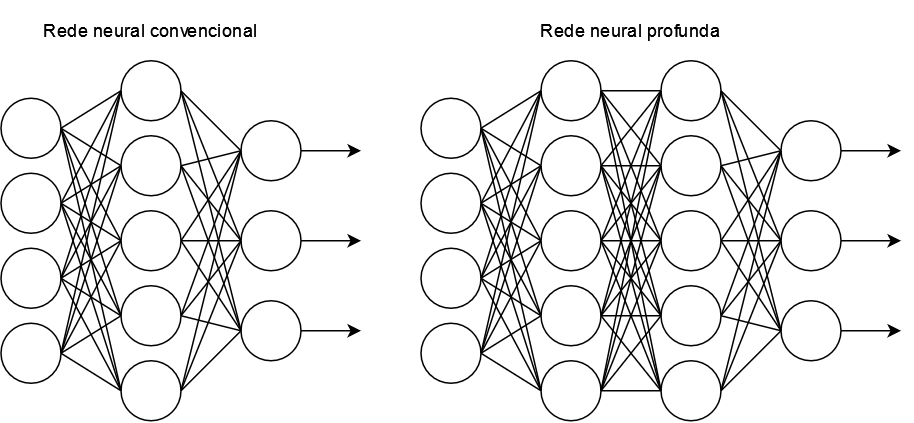
\includegraphics[width=0.8\textwidth]{figures/redes_neurais.png}
	\caption{Comparação de uma rede neural convencional com uma rede neural profunda.}	
	\label{fig:redes_neurais}
\end{figure}

\subsection{Redes neurais convolucionais}
Uma rede neural convolucional é análoga à rede neural artificial, i.e., feita de neurônios que otimizam o aprendizado através dele mesmo. A principal diferença é que a rede neural convolucional é amplamente utilizada em soluções que detectam padrões em imagens, logo existem funcionalidades específicas da própria arquitetura para essa tarefa \cite{oshea2015introduction}.

De acordo com \citeonline{dp_overview}, uma arquitetura básica de uma rede neural convolucional tem as seguintes camadas: convolucional, pooling e totalmente conectada.

\begin{figure}[H]
	\caption{Camadas principais de uma rede neural convolucional}
	\centering % para centralizarmos a figura
	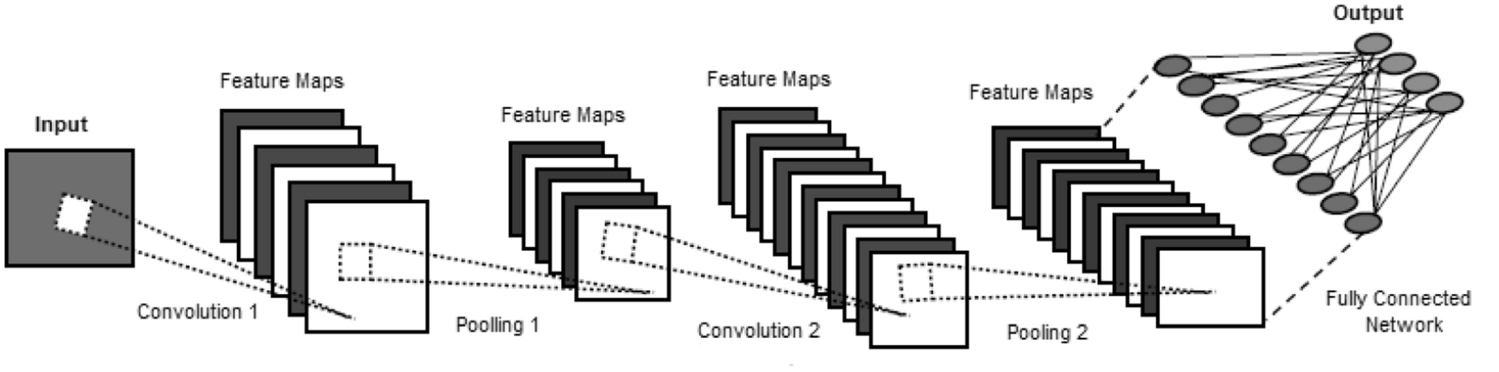
\includegraphics[width=15cm]{figures/arquitetura_cnn.png} % leia abaixo
	\legend{Fonte: \citeonline{dp_overview}}
	\label{fig:arquitetura_cnn}
\end{figure}

Camada convolucional é essencial para esse tipo de arquitetura e usa um filtro — ou kernel — para aplicar na imagem e direcionar para o próximo neurônio. Esse filtro é uma matriz de números que terá uma operação aplicada em todos os píxeis da imagem — que também é representado por matriz(es) — as informações cruciais para esse filtro são: tamanho, largura e pesos. Isto é utilizado para extrair características com uma base matemática, criando uma relação direta entre um píxel e os píxeis ao redor. Os pesos começam de forma pseudoaleatórias e são ajustados no decorrer do aprendizado. O resultado dessa camada é chamado de mapa de características.

O tamanho da saída será baseado na fórmula abaixo sendo os tamanhos I da imagem, F do filtro e a S da saída.

$$
\begin{aligned}
\mathbf{I}x - \mathbf{F}x + 1 &= \mathbf{S}x \\
\mathbf{I}y - \mathbf{F}y + 1 &= \mathbf{S}y
\end{aligned}
$$

\begin{figure}[H]
	\caption{Exemplo de um filtro}
	\centering % para centralizarmos a figura
	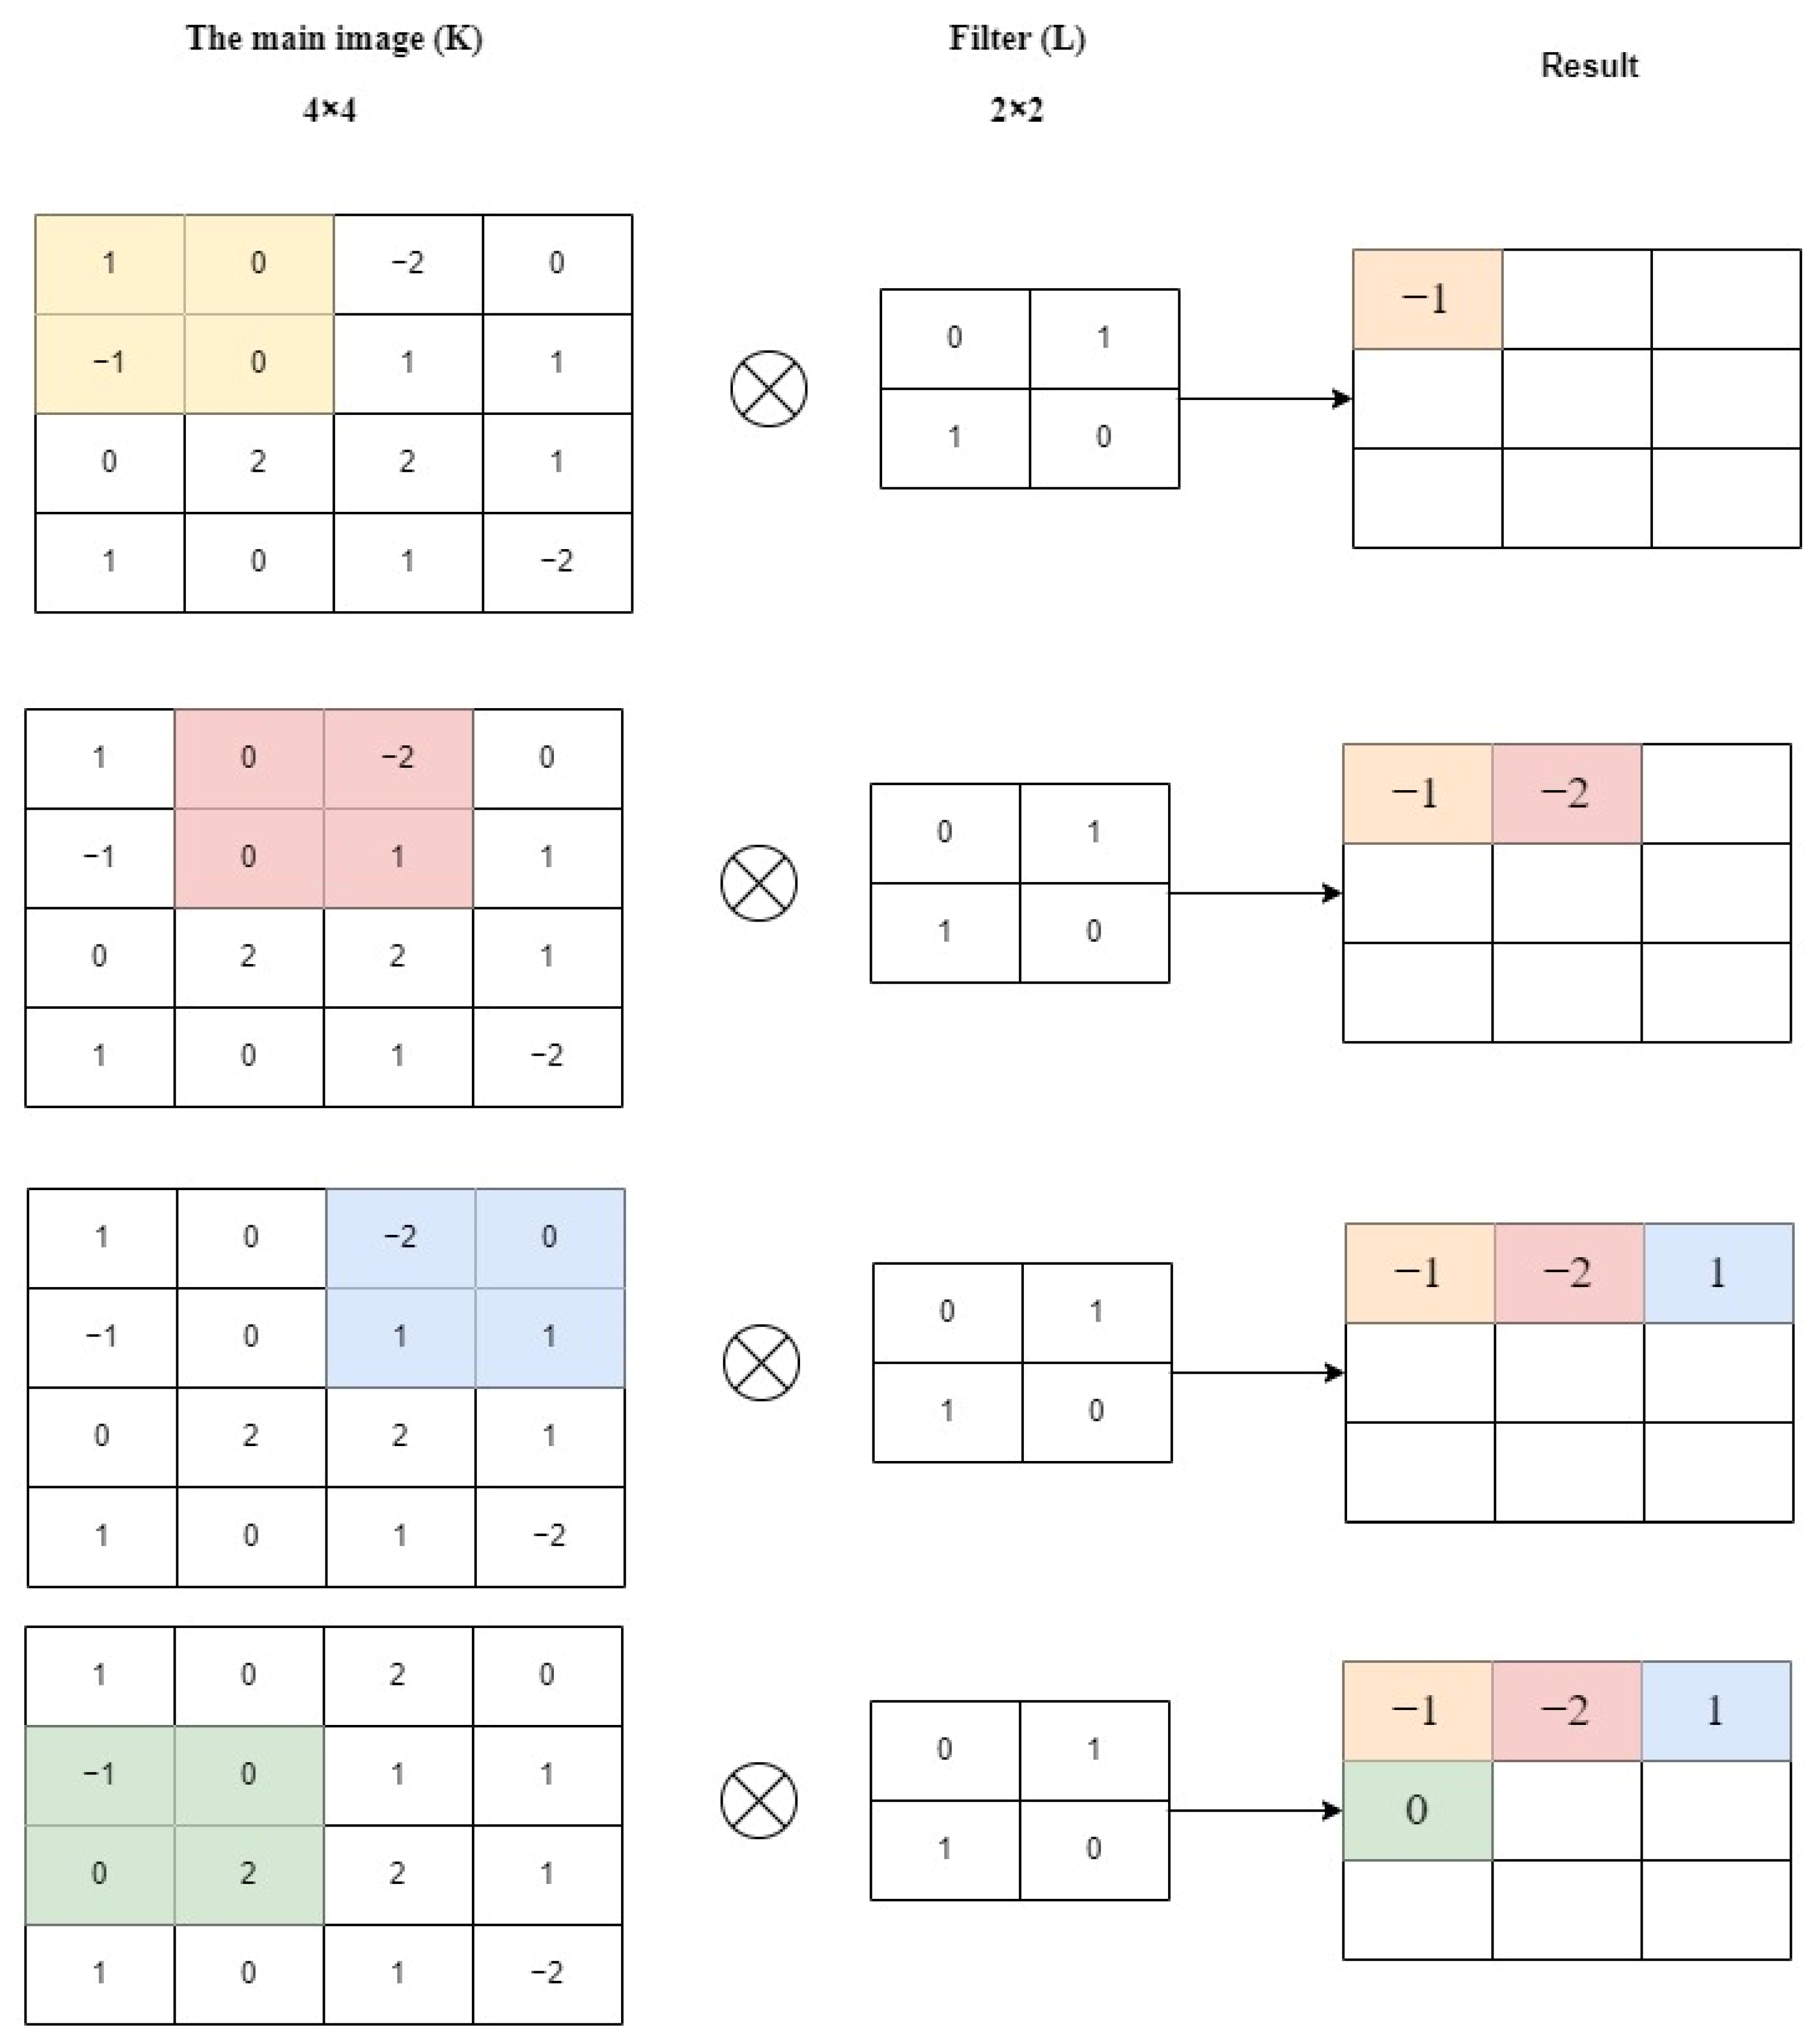
\includegraphics[width=10cm]{figures/exemplo_filtro.png} % leia abaixo
	\legend{Fonte: \citeonline{computation11030052}}
	\label{fig:exeplo_filtro}
\end{figure}

A camada de pooling tem como tarefa primordial uma técnica para reduzir o tamanho do mapa de características porém preservando os padrões mais relevantes. Dentre os recursos essenciais dessa camada estão o tamanho do pooling e a operação que será realizada. Dentre vários tipos de pooling os mais utilizados são: pooling máximo, pooling médio e pooling global médio \cite{Alzubaidi2021}. 

$\textbf{Pooling médio}$

É definido o resultado final com base na média encontrada pelo tamanho do pooling, exemplo a seguir usando um mapa de características com tamanho 4x4 e pooling de tamanho 2x2.

$$
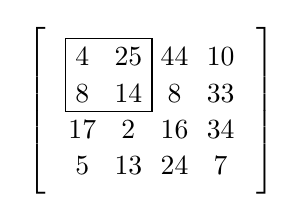
\begin{tikzpicture}[baseline=-0.5ex]
    \matrix (M) [matrix of math nodes,left delimiter={[},right delimiter={]}] {
        4 & 25 & 44 & 10\\
        8 & 14 & 8 & 33 \\
        17 & 2 & 16 & 34 \\
        5 & 13 & 24 & 7 \\
    };
    \draw (M-1-1.north west) rectangle (M-2-2.south east);
\end{tikzpicture}
= 
\begin{bmatrix}
	\boxed{12} & 23 \\
	9 & 20 \\
   \end{bmatrix}
$$

$\textbf{Pooling máximo}$

É definido o resultado final com base no máximo encontrado pelo tamanho do pooling, exemplo a seguir usando um mapa de características com tamanho 4x4 e pooling de tamanho 2x2.

$$
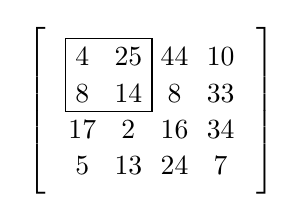
\begin{tikzpicture}[baseline=-0.5ex]
    \matrix (M) [matrix of math nodes,left delimiter={[},right delimiter={]}] {
        4 & 25 & 44 & 10\\
        8 & 14 & 8 & 33 \\
        17 & 2 & 16 & 34 \\
        5 & 13 & 24 & 7 \\
    };
    \draw (M-1-1.north west) rectangle (M-2-2.south east);
\end{tikzpicture}
= 
\begin{bmatrix}
	\boxed{25} & 44 \\
	17 & 34 \\
   \end{bmatrix}
$$

$\textbf{Pooling global médio}$

É definido o resultado final com base na média geral do mapa o que sempre tem como saída uma matrix 1x1, exemplo a seguir usando um mapa de características com tamanho 4x4.

$$
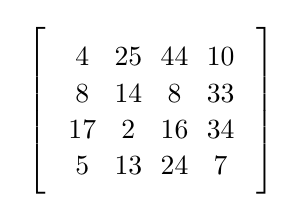
\begin{tikzpicture}[baseline=-0.5ex]
    \matrix (M) [matrix of math nodes,left delimiter={[},right delimiter={]}] {
        4 & 25 & 44 & 10\\
        8 & 14 & 8 & 33 \\
        17 & 2 & 16 & 34 \\
        5 & 13 & 24 & 7 \\
    };
\end{tikzpicture}
= 
\begin{bmatrix}
	16
   \end{bmatrix}
$$

\subsection{Visão computacional}
A visão computacional avança cada vez mais, aproximando os computadores da capacidade visual humana.Segundo Horst Haußecker e Bernd Jähne no livro "Computer Vision and Applications" \cite{comp_vision_and_applications}, a visão computacional é uma área da computação que se dedica à interpretação de imagens por meio de algoritmos e técnicas de processamento de imagens. Essa área abrange a aquisição, processamento e análise de imagens, com o objetivo de extrair informações úteis para resolver problemas específicos.

A visão é um elemento crucial para capacitar a inteligência artificial a realizar diversas tarefas. A fim de replicar a visão humana, é necessário que as máquinas sejam capazes de adquirir, processar, analisar e compreender imagens. \cite{como_funciona_visao_computacional}

Na \cref{fig:comp_vision} podemos ver uma analogia entre a forma como uma imagem é processada pelo cérebro humano e a forma como é processada por um sistema computacional.

\begin{figure}[!ht]
	\centering
	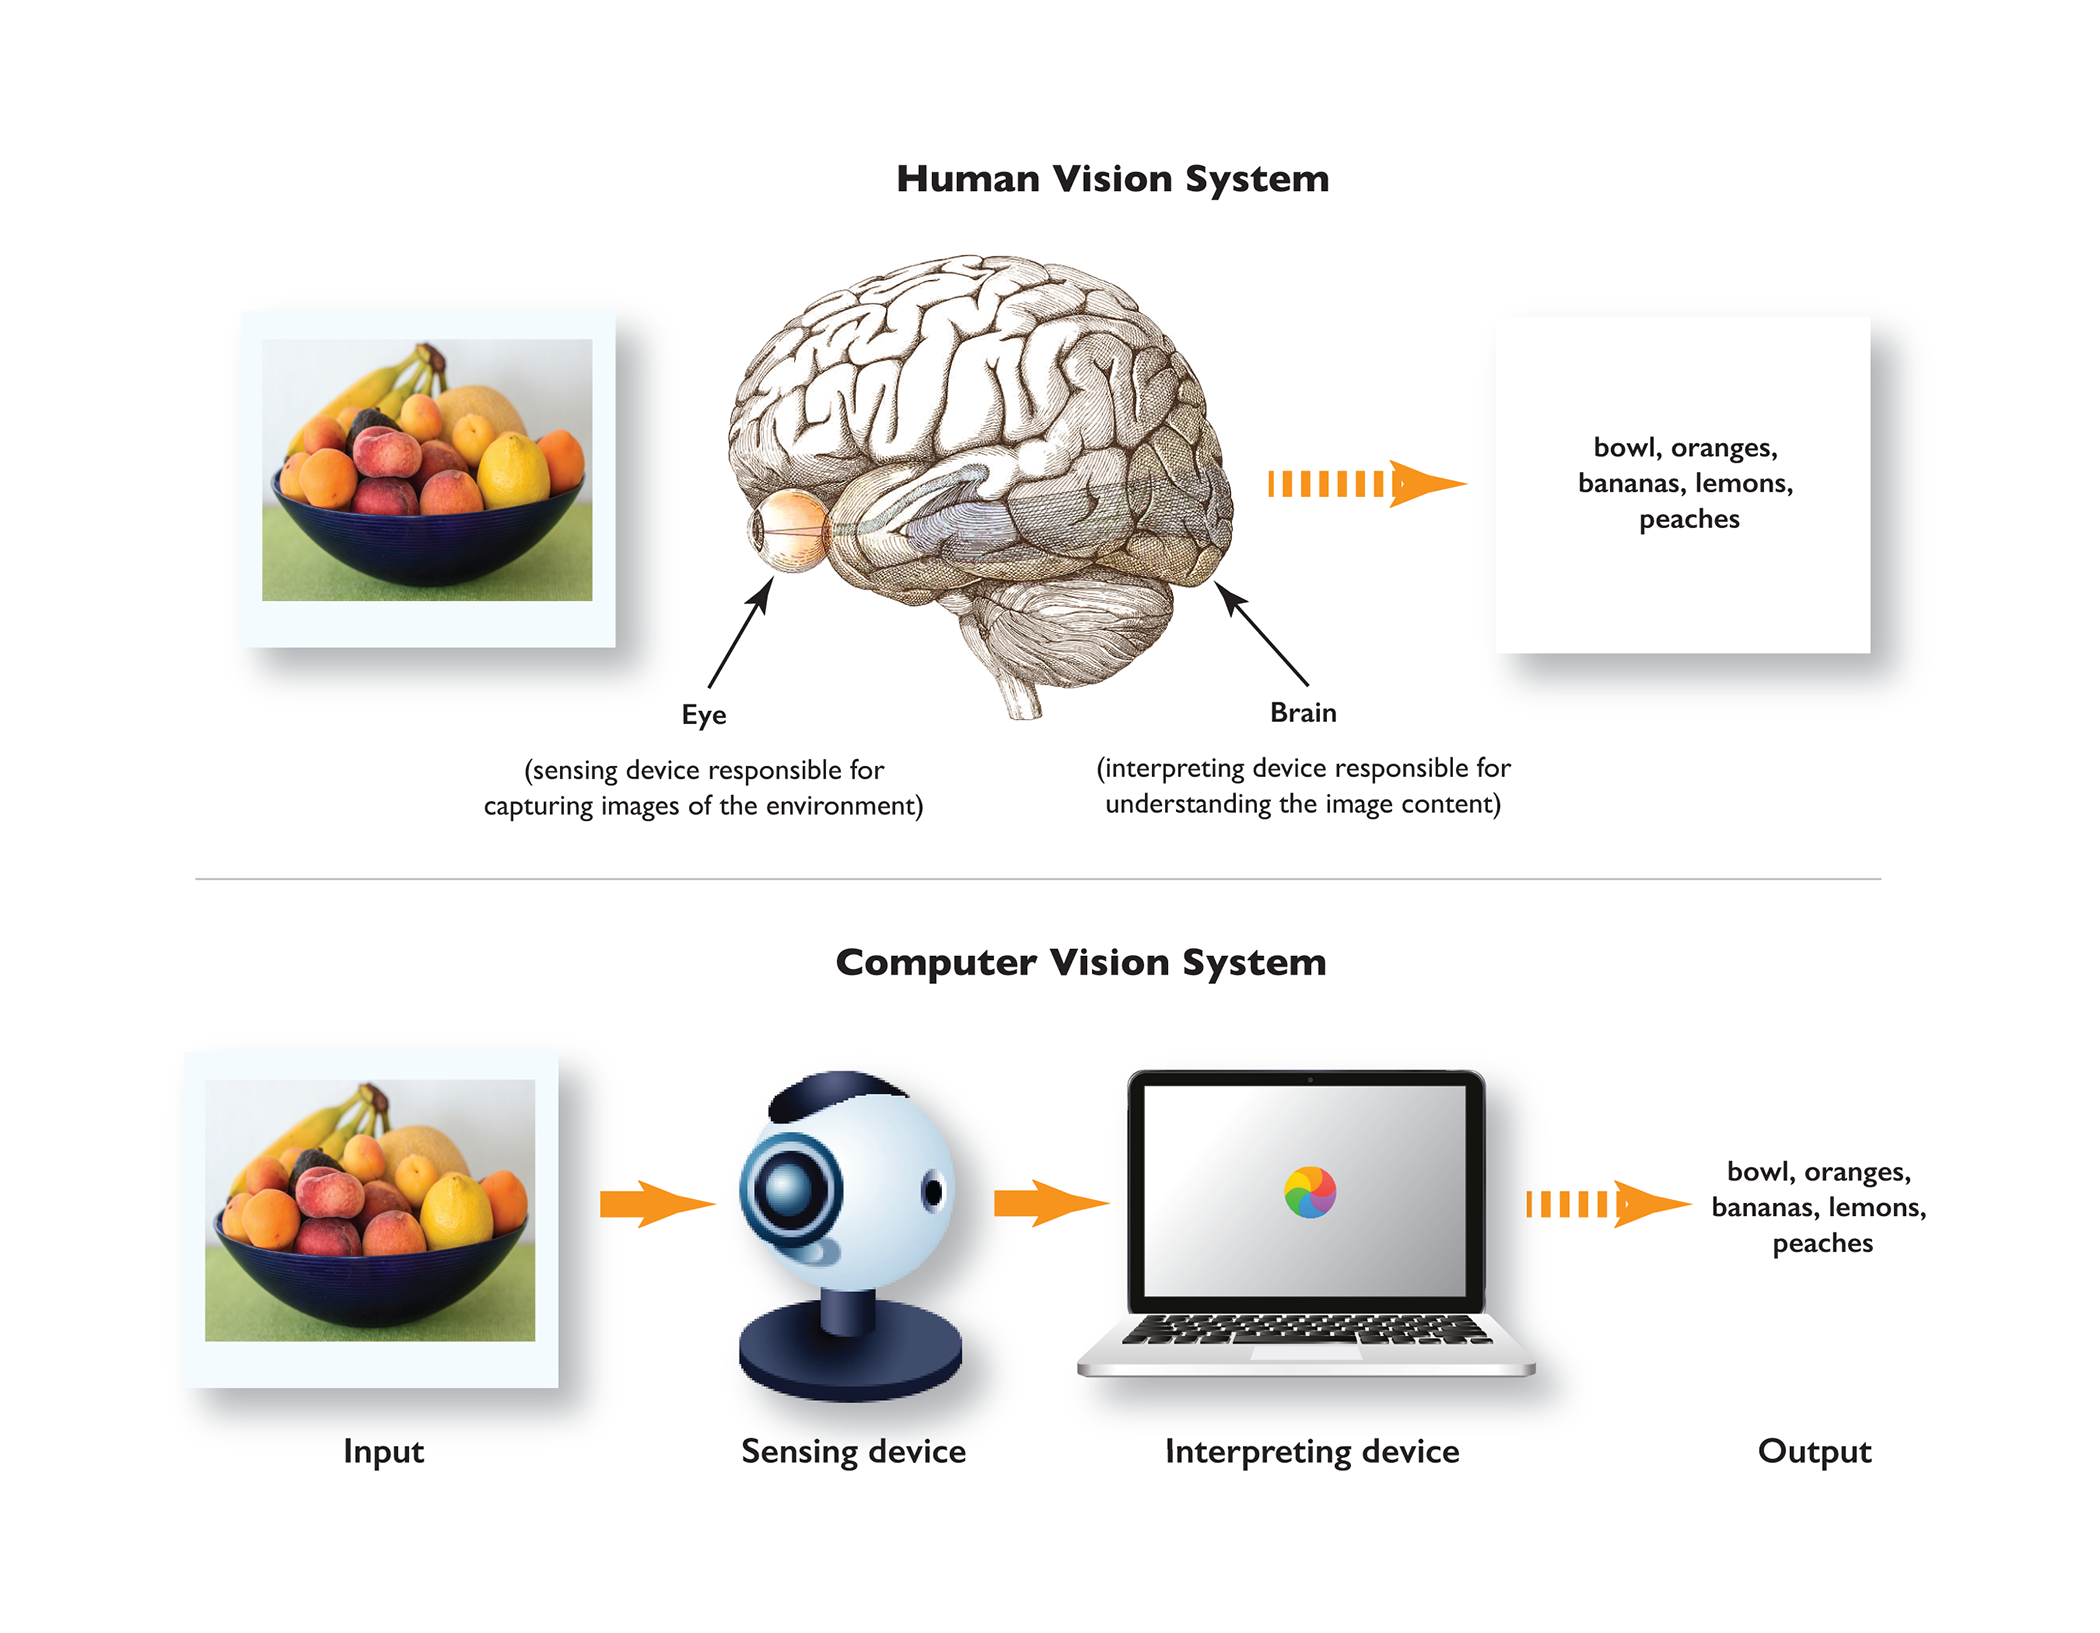
\includegraphics[width=0.6\textwidth]{figures/content_Human_Vision.png}
	\caption{Comparação entre a forma de como o cérebro humano e um computador processam informações \cite{content_Human_Vision}.}
	\label{fig:comp_vision}
\end{figure}	

\subsubsection{Pré-processamento de Imagens}

\subsubsection{Detectação de objetos}

\subsubsection{Segmentação de imagem}

\subsection{Algoritmos de segmentação}

\section{Geração procedural}
\subsection{Diagrama de Voronoi}

O diagrama de Voronoi é gerado a partir das distancias euclidianas entre os vizinhos mais próximos de um conjunto de pontos do plano\space
\cite{diagrama_de_voronoi:_uma_exploracao_nas_distancias_euclidiana_e_do_taxi}. Esse diagrama possui uma gama de utilizações, por exemplo, estudar epidemias, encontrar o 
ponto mais próximo, calcular a precipitação de uma área, estudar os padrões de crescimento das florestas, etc,\space\cite{poligonos_de_thiessen_ou_voronoi}. 

Seja um conjunto de índices $I_n = \{1, 2, 3, ..., n\}$ e $A = \{p_1, p_2, ..., p_n\} \subset \mathbb{R}^2$ um conjunto de pontos onde $2 \leq n < \infty$, definimos como região de Voronoi o conjunto de pontos associado a $p_i$, onde d é a distancia euclidiana

$$V(p_i) = \{p|d(p_i,p) \leq d(p_i,p);i \neq j, i, j \in I_n\},$$

temos o conjunto formado por essas regiões sendo $V(A) = {V(1), V(2), V(3), ..., V(n)}$ \cite{rodrigues_diagrama_2019}.

Na figura \cref{fig:diagrama_voronoi} podemos ver a relação do conjuntos de pontos com o diagrama de Voronoi.
\begin{figure}[H]
	\centering
	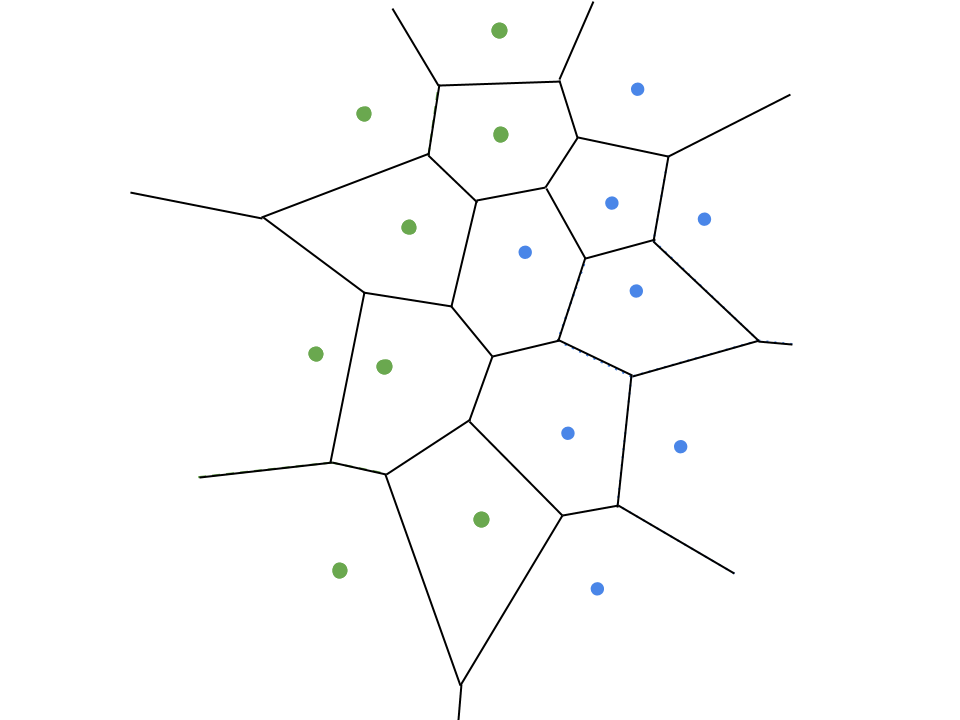
\includegraphics[width=0.8\textwidth]{figures/diagrama_de_voronoi.png}
	\caption{Diagrama de Voronoi \cite{thomazthz_diagrama_2014}.}	
	\label{fig:diagrama_voronoi}
\end{figure}



\section{Trabalhos relacionados}
Esta seção destina-se a análise e discussão da metodologia e dos resultados prospostos por \citeonline{geracao_procedural_jogos_2d}. 

\subsection{Geração Procedural de Mapas para Jogos 2D}

No trabalho \citeonline{geracao_procedural_jogos_2d}, é apresentado uma solução simples para criar mapas de cavernas, calabouços e ilhas para jogos 2D. O algoritmo foi dividido em três partes sendo elas: geração recursiva de terrenos, validação de tamanho e correção da coesão. Os autores concluíram que não existe literatura sobre geração procedural de salas diversas e corredores distintos como o algoritmo proposto. Sugerem duas possibilidades para trabalhos futuros sendo elas: usar algoritmos genéticos para mensurar a qualidade dos mapas gerados e promover pela seleção natural e a outra possibilidade é mesclar o algoritmo proposto com técnicas de geração de salas interligadas por corredores, de forma a possibilitar a criação de mapas com algumas salas pré-definidas inseridas em um mapa aberto contínuo.

\chapter{Desenvolvimento}

% ----------------------------------------------------------
% Finaliza a parte no bookmark do PDF
% para que se inicie o bookmark na raiz
% e adiciona espaço de parte no Sumário
% ----------------------------------------------------------
%\phantompart

% ---
% Conclusão (outro exemplo de capítulo sem numeração e presente no sumário)
% ---
\chapter*[Conclusão]{Conclusão}
\addcontentsline{toc}{chapter}{Conclusão}
% ---

\lipsum[31-33]

% ----------------------------------------------------------
% ELEMENTOS PÓS-TEXTUAIS
% ----------------------------------------------------------
\postextual
% ----------------------------------------------------------

% ----------------------------------------------------------
% Referências bibliográficas
% ----------------------------------------------------------
\bibliography{references}

% ----------------------------------------------------------
% Glossário
% ----------------------------------------------------------
%
% Consulte o manual da classe abntex2 para orientações sobre o glossário.
%
%\glossary

% ----------------------------------------------------------
% Apêndices
% ----------------------------------------------------------

% ---
% Inicia os apêndices
% ---
% \begin{apendicesenv}

% % Imprime uma página indicando o início dos apêndices
% \partapendices

% % ----------------------------------------------------------
% \chapter{Quisque libero justo}
% % ----------------------------------------------------------

% \lipsum[50]

% % ----------------------------------------------------------
% \chapter{Nullam elementum urna vel imperdiet sodales elit ipsum pharetra ligula
% ac pretium ante justo a nulla curabitur tristique arcu eu metus}
% % ----------------------------------------------------------
% \lipsum[55-57]

% \end{apendicesenv}
% ---


% ----------------------------------------------------------
% Anexos
% ----------------------------------------------------------

% ---
% Inicia os anexos
% ---
% \begin{anexosenv}

% % Imprime uma página indicando o início dos anexos
% \partanexos

% % ---
% \chapter{Morbi ultrices rutrum lorem.}
% % ---
% \lipsum[30]

% % ---
% \chapter{Cras non urna sed feugiat cum sociis natoque penatibus et magnis dis
% parturient montes nascetur ridiculus mus}
% % ---

% \lipsum[31]

% % ---
% \chapter{Fusce facilisis lacinia dui}
% % ---

% \lipsum[32]

% \end{anexosenv}

%---------------------------------------------------------------------
% INDICE REMISSIVO
%---------------------------------------------------------------------
%\phantompart
\printindex
%---------------------------------------------------------------------

\end{document}